\documentclass[submission]{grattan}
%\documentclass[a4paper,11pt]{scrreprt}
\usepackage{amsmath}
\usepackage{amssymb}
\usepackage{tikz}
\usepackage{url}
%\usepackage{lmodern}
\usepackage{microtype}

\newcommand*{\code}[1]{\texttt{#1}}
\newcommand*{\defi}[1]{\textbf{#1}}

\addbibresource{bib/Grattan-Master-Bibliography.bib}

\ReportOrWorkingPaper{WorkingPaper}
\GrattanReportNumber{2019-00}
\MONTH{July}

\title{Technical supplement to the COVID19 report}
\author{Hugh Parsonage}

\providecommand{\crema}{\textsc{crema}}

% ignore_spelling_in: code
% add_to_dictionary: SupermarketTypical Lehmer Lemire OpenMP lockdowns? infectors caf es



\begin{document}
\contentspage

\chapter{Overview and scope}\label{chap:tech-supp-overview}
Our model, \crema, is a dynamic microsimulation model of Australia.
The model is written in R and Rcpp.

The purpose of the model is to show the effect of policy changes on the spread of infections 
throughout Australia, under a flexible 
set of epidemiological assumptions about the disease. By necessity, the model also
`nowcasts' the number of active cases from official reports of new infections and
their sources. 

\crema\ does not model the effect of overseas arrivals, only new infections
arising from local transmission. It also does not estimate new infections arising
from breaches of quarantine.  While a large majority of Australia's COVID-19 cases 
arose from these sources, the policy response to these threats was not contentious.

\begin{figure}
\caption{Most new infections were from new arrivals, or coincided with the peak in overseas cases}\label{fig:nsw-sources}
\units{New cases, by source}
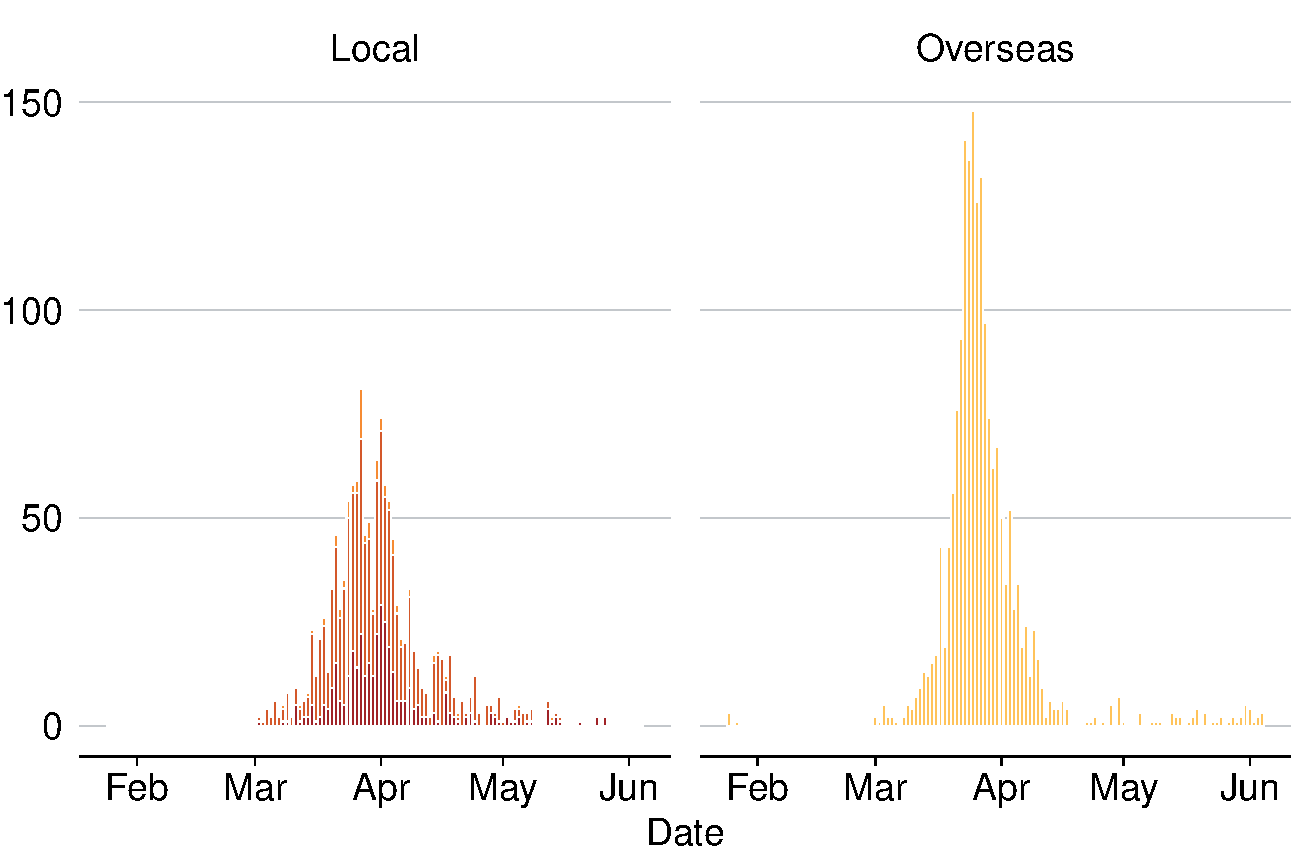
\includegraphics{atlas/nsw-sources.pdf}
\source{(pappubahry)}
\end{figure}

\section{Static data}
The model runs on a static data table, each row a person in Australia,
which identifies each person's

\begin{enumerate}
	\item state and SA2,
	\item age,
	\item household,
	\item school, and
	\item labour force status.
\end{enumerate}

For performance reasons, data is cached before being passed to the dynamic model.
Obviously, the cache includes the static data. Other features of each person is
also cached (or ``generated at cache time''). 

The other cache time variables are \code{SupermarketTypical} and the workplace variables.
For \code{SupermarketTypical},
if an individual's SA2 contains zero supermarkets,
a value of zero.
For implementation convenience,%
	\footnote{By \defi{implementation convenience}, I mean that the choice was not made
	on the basis of research, because it was necessary to do so and was not considered
	sufficiently important to make more than an arbitrary decision. In this case,
	the choice of 8 was made to avoid stack overflow.}
if the individual's SA2 contains more than eight supermarket we
exclude all but eight supermarkets. We then randomly assign each person to 
a `typical' supermarket for the person to visit during the model run.


\subsection{Assignment of individuals to workplaces}
While we are confident about the distribution of labour force status among
the population we assign in the static data, we do not know how large each
worker's workplace is. To model this, for each destination zone we construct
a sequence of geometrically distributed random variables with parameters
\(1/\beta = 1/15\).

\begin{figure}[!htbp]
\caption{The geometric distribution with mean 15 over [0, 50]}\label{fig:geom-distr}
% \makebox[\textwidth]{
\par
	% Created by tikzDevice version 0.12.3 on 2020-06-05 12:24:45
% !TEX encoding = UTF-8 Unicode
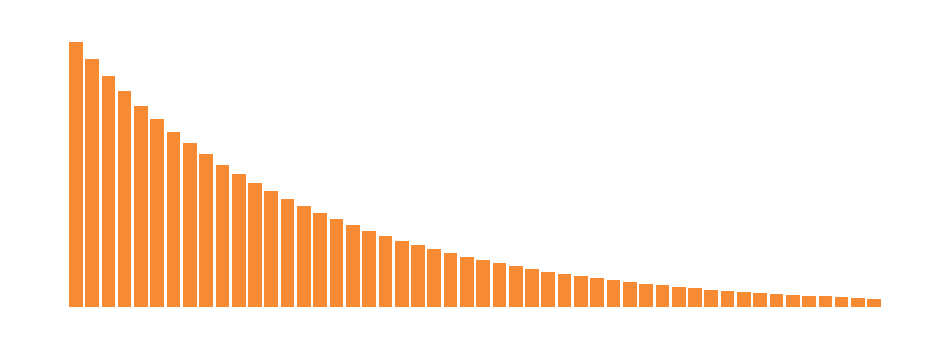
\begin{tikzpicture}[x=1pt,y=1pt]
\definecolor{fillColor}{RGB}{255,255,255}
\path[use as bounding box,fill=fillColor,fill opacity=0.00] (0,0) rectangle (323.21,105.74);
\begin{scope}
\path[clip] (  0.00,  0.00) rectangle (323.21,105.74);
\definecolor{drawColor}{RGB}{255,255,255}
\definecolor{fillColor}{RGB}{246,139,51}

\path[draw=drawColor,line width= 0.3pt,line cap=rect,fill=fillColor] ( 14.69,  4.81) rectangle ( 19.99,100.94);

\path[draw=drawColor,line width= 0.3pt,line cap=rect,fill=fillColor] ( 20.58,  4.81) rectangle ( 25.88, 94.53);

\path[draw=drawColor,line width= 0.3pt,line cap=rect,fill=fillColor] ( 26.47,  4.81) rectangle ( 31.77, 88.55);

\path[draw=drawColor,line width= 0.3pt,line cap=rect,fill=fillColor] ( 32.36,  4.81) rectangle ( 37.66, 82.96);

\path[draw=drawColor,line width= 0.3pt,line cap=rect,fill=fillColor] ( 38.24,  4.81) rectangle ( 43.54, 77.75);

\path[draw=drawColor,line width= 0.3pt,line cap=rect,fill=fillColor] ( 44.13,  4.81) rectangle ( 49.43, 72.89);

\path[draw=drawColor,line width= 0.3pt,line cap=rect,fill=fillColor] ( 50.02,  4.81) rectangle ( 55.32, 68.35);

\path[draw=drawColor,line width= 0.3pt,line cap=rect,fill=fillColor] ( 55.91,  4.81) rectangle ( 61.21, 64.11);

\path[draw=drawColor,line width= 0.3pt,line cap=rect,fill=fillColor] ( 61.80,  4.81) rectangle ( 67.10, 60.16);

\path[draw=drawColor,line width= 0.3pt,line cap=rect,fill=fillColor] ( 67.69,  4.81) rectangle ( 72.99, 56.47);

\path[draw=drawColor,line width= 0.3pt,line cap=rect,fill=fillColor] ( 73.57,  4.81) rectangle ( 78.87, 53.03);

\path[draw=drawColor,line width= 0.3pt,line cap=rect,fill=fillColor] ( 79.46,  4.81) rectangle ( 84.76, 49.81);

\path[draw=drawColor,line width= 0.3pt,line cap=rect,fill=fillColor] ( 85.35,  4.81) rectangle ( 90.65, 46.81);

\path[draw=drawColor,line width= 0.3pt,line cap=rect,fill=fillColor] ( 91.24,  4.81) rectangle ( 96.54, 44.01);

\path[draw=drawColor,line width= 0.3pt,line cap=rect,fill=fillColor] ( 97.13,  4.81) rectangle (102.43, 41.40);

\path[draw=drawColor,line width= 0.3pt,line cap=rect,fill=fillColor] (103.02,  4.81) rectangle (108.31, 38.96);

\path[draw=drawColor,line width= 0.3pt,line cap=rect,fill=fillColor] (108.90,  4.81) rectangle (114.20, 36.68);

\path[draw=drawColor,line width= 0.3pt,line cap=rect,fill=fillColor] (114.79,  4.81) rectangle (120.09, 34.56);

\path[draw=drawColor,line width= 0.3pt,line cap=rect,fill=fillColor] (120.68,  4.81) rectangle (125.98, 32.57);

\path[draw=drawColor,line width= 0.3pt,line cap=rect,fill=fillColor] (126.57,  4.81) rectangle (131.87, 30.72);

\path[draw=drawColor,line width= 0.3pt,line cap=rect,fill=fillColor] (132.46,  4.81) rectangle (137.76, 28.99);

\path[draw=drawColor,line width= 0.3pt,line cap=rect,fill=fillColor] (138.34,  4.81) rectangle (143.64, 27.38);

\path[draw=drawColor,line width= 0.3pt,line cap=rect,fill=fillColor] (144.23,  4.81) rectangle (149.53, 25.88);

\path[draw=drawColor,line width= 0.3pt,line cap=rect,fill=fillColor] (150.12,  4.81) rectangle (155.42, 24.47);

\path[draw=drawColor,line width= 0.3pt,line cap=rect,fill=fillColor] (156.01,  4.81) rectangle (161.31, 23.16);

\path[draw=drawColor,line width= 0.3pt,line cap=rect,fill=fillColor] (161.90,  4.81) rectangle (167.20, 21.94);

\path[draw=drawColor,line width= 0.3pt,line cap=rect,fill=fillColor] (167.79,  4.81) rectangle (173.09, 20.80);

\path[draw=drawColor,line width= 0.3pt,line cap=rect,fill=fillColor] (173.67,  4.81) rectangle (178.97, 19.73);

\path[draw=drawColor,line width= 0.3pt,line cap=rect,fill=fillColor] (179.56,  4.81) rectangle (184.86, 18.73);

\path[draw=drawColor,line width= 0.3pt,line cap=rect,fill=fillColor] (185.45,  4.81) rectangle (190.75, 17.81);

\path[draw=drawColor,line width= 0.3pt,line cap=rect,fill=fillColor] (191.34,  4.81) rectangle (196.64, 16.94);

\path[draw=drawColor,line width= 0.3pt,line cap=rect,fill=fillColor] (197.23,  4.81) rectangle (202.53, 16.13);

\path[draw=drawColor,line width= 0.3pt,line cap=rect,fill=fillColor] (203.12,  4.81) rectangle (208.42, 15.38);

\path[draw=drawColor,line width= 0.3pt,line cap=rect,fill=fillColor] (209.00,  4.81) rectangle (214.30, 14.67);

\path[draw=drawColor,line width= 0.3pt,line cap=rect,fill=fillColor] (214.89,  4.81) rectangle (220.19, 14.01);

\path[draw=drawColor,line width= 0.3pt,line cap=rect,fill=fillColor] (220.78,  4.81) rectangle (226.08, 13.40);

\path[draw=drawColor,line width= 0.3pt,line cap=rect,fill=fillColor] (226.67,  4.81) rectangle (231.97, 12.83);

\path[draw=drawColor,line width= 0.3pt,line cap=rect,fill=fillColor] (232.56,  4.81) rectangle (237.86, 12.29);

\path[draw=drawColor,line width= 0.3pt,line cap=rect,fill=fillColor] (238.45,  4.81) rectangle (243.75, 11.79);

\path[draw=drawColor,line width= 0.3pt,line cap=rect,fill=fillColor] (244.33,  4.81) rectangle (249.63, 11.33);

\path[draw=drawColor,line width= 0.3pt,line cap=rect,fill=fillColor] (250.22,  4.81) rectangle (255.52, 10.89);

\path[draw=drawColor,line width= 0.3pt,line cap=rect,fill=fillColor] (256.11,  4.81) rectangle (261.41, 10.49);

\path[draw=drawColor,line width= 0.3pt,line cap=rect,fill=fillColor] (262.00,  4.81) rectangle (267.30, 10.11);

\path[draw=drawColor,line width= 0.3pt,line cap=rect,fill=fillColor] (267.89,  4.81) rectangle (273.19,  9.75);

\path[draw=drawColor,line width= 0.3pt,line cap=rect,fill=fillColor] (273.78,  4.81) rectangle (279.07,  9.42);

\path[draw=drawColor,line width= 0.3pt,line cap=rect,fill=fillColor] (279.66,  4.81) rectangle (284.96,  9.12);

\path[draw=drawColor,line width= 0.3pt,line cap=rect,fill=fillColor] (285.55,  4.81) rectangle (290.85,  8.83);

\path[draw=drawColor,line width= 0.3pt,line cap=rect,fill=fillColor] (291.44,  4.81) rectangle (296.74,  8.56);

\path[draw=drawColor,line width= 0.3pt,line cap=rect,fill=fillColor] (297.33,  4.81) rectangle (302.63,  8.31);

\path[draw=drawColor,line width= 0.3pt,line cap=rect,fill=fillColor] (303.22,  4.81) rectangle (308.52,  8.08);
\end{scope}
\end{tikzpicture}

% }
\end{figure}

The number of random variables to generate is determined algorithmically: if the next random variable
would overflow into the next DZN, we fill the rest of the sequences with 2, which has the useful
side-effect of inflating the number of partnerships to a number consistent with observation.
With this sequence we obtain, for each working person, a group of workers associated with each person
and the size of their workplace.

Assignment of workplace information completes the data generated at cache time. All other personal
features are constructed anew at runtime.

\section{Assignment of candidate incubation and illness }

Our next step is to construct vectors to reflect user-supplied epidemiological parameters.
We construct for each person the duration of their incubation period and illness should they
be infected when the model starts. Although it would seem wasteful to generate these values
for every person, even if only a fraction of a percent of the rows are likely to be used, it
so happens that this is more efficient than constructing them `just-in-time', mostly because
the model can perform large parts of its operation across the population in parallel, during
which time the generation of random numbers is more difficult to coordinate.

The generation of the Poisson and log-normal distributions are done in the normal way using
 standard functions from the \code{stats} package.  For efficiency, we construct a small vector
 then use \code{rep\_len} to replicate it along the height of the data table. For example, if
 a Poisson distribution with parameter \(\lambda = 5\) is requested, we construct the vector

\[\text{\code{rep\_len(rpois(131059, 5), nrow(aus))}} \]

 For the Cauchy distribution, we implement our own version to allow for parallelized random
 number generation with an R seed. The Cauchy distribution is characterized by infrequent
 extreme values so taking a small sample and repeating it was not adequate for this task.
 Since the Cauchy distribution has support over negative values,
 we use the absolute value.

 In addition, we construct a \defi{Resistance} vector which assigns a integer value from 0-1000
 for each person. These values combined with a parameter \code{resistance\_threshold} simulate
 natural resistance throughout the population: persons whose \code{Resistance[i]} exceeds
 the user-supplied \code{resistance\_threshold} do not get infected, even if they come into 
 contact with an infectious person. 

\subsection{Reconstructing patient histories from the starting point}
The model accepts a starting date as an input, as an alternative to supplying the
number and distribution of active and inactive cases in the population.
 To determine the number of active and inactive cases from a given starting date,
 we use a time series of each state's cumulative cases, together with assumptions
 about the source of each infection, and the epidemiological parameters that govern
 the duration of each persons' illness.%
 	\footnote{The time series data is from \url{https://github.com/pappubahry/AU_COVID19}, who
 	compiled the data from the state and territory health departments.}
 While some states
 	report recoveries and sources of infections, this information is not reported consistently
 	 (if at all) throughout the period.
Hence we are only able to \emph{estimate} the number of active cases at a point in time,
even if we take the data at face value. We assume that the cumulative number of cases
by date is correct, and we use the day-on-day difference of this number to reckon the
number of new cases. To each new case we assign a random member of the state's population and,
using the incubation and illness vectors allocated previously, determine the dates on which
the case was active.

Since a large number of new cases were from overseas arrivals, and since such individuals are more
likely to be quarantined from the population, we also need to estimate how many of the
above cases would be in quarantine (and thus excluded from the model). We use the NSW and
Victorian time series of infection sources to impute an overall percentage of new cases
on a given date that would be isolated and apply this percentage to all new cases to
determine the number of new cases that exist in the wider community. On certain dates,
in certain states,
the number of cases reported to have an overseas origin appears to exceed the \emph{total}
number of cases. In addition, the number of overseas cases is higher for earlier dates and
becomes a less common source of infection after March. To moderate these effects, we subtract
the corresponding numbers of recovered patients in NSW and Victoria from both the number of
overseas infections and the number of infections overall. We then take the average of the
two percentages as the overall percentage of quarantined new infections on a particular date.
The number of deaths at the starting point is determined by the time series of deaths by state.

Otherwise, if the \code{InitialStatus} input is set, it is used to construct the initial status directly.

\section{Pseudo random number generator}

Like most models of this nature, random number generation is both a core element and
a performance bottleneck.  We use a
pseudo random number generator (PRNG) devised by Lehmer:\footnote{\url{https://lemire.me/blog/2019/03/19/the-fastest-conventional-random-number-generator-that-can-pass-big-crush/}.}

\[ \frac{x \mapsto(x \times 15750249268501108736)}{2^{64}}\]

The simplicity in the formulation makes seeding and parallelism relatively straightforward. We
initialize the PRNG with a state space of twenty 128-bit integers
and simply cap the number of threads at twenty whenever
the PRNG is used. This array is seeded before each day, using R's PRNG's default state, the integer
vector \code{.Random.seed} via
the \code{dqrng} package.

When the user requests single-threaded operations, a single 128-bit integer is used for
the state and seeded in the same technique as Lemire.

 To obtain Bernoulli random variables
(as when applying transmission
probabilities), we unpack the random number into \code{unsigned char} values as required.
This approach reduces the loop iteration by a factor of eight, though leads to data dependencies
within each pack (indeed along adjacent packs or every sixteen numbers). While this weakens
the randomness of transmission probabilities among adjacent persons, this lack of
independence dwarfed by the simulation's dependence on the precise initial state. Since the only way
to reduce errors arising from unlucky choices of initial state (such as all infectious cases occurring
in a single suburb, or all infectious individuals being in single-person households) is to increase
the raw number of simulations, the performance gains were deemed to be worth this infelicity.

Although most of the parallelism is embarrassingly parallel or simple reductions, we expect the OpenMP
compiler to statically allocate threads, which should maintain the reproducibility of results. A more
thorough approach to reproducible PRNGs would be to statically allocate threads.



\section{Infection model}

At the start of each day, various properties of the current state of the population is recorded,
depending on the return type selected. In all cases, the number of active cases is recorded.
If the number of active cases reaches zero, or the number of days to simulate is reached, the model
 terminates and these daily summaries returned.

Each person has a \textbf{Status} which is a 32-bit signed integer indicating whether or not
they are infected or have been infected, whether or not they are in isolation, and whether they are
in intensive care. A status of zero indicates the person is susceptible to infection (but not
in isolation). Negative values indicate the person had been infected previously. Individuals with
negative statuses cannot be reinfected.


If an age-based lockdown is selected, the status of  all individuals of the ages requested have their
status flagged as isolated.

All infected individuals are then moved either from an incubation period to one of
`symptomatic' or `critical', or from one of those status to `healed' or `killed', based
on the precomputed prognosis.

Next, the person-to-person infection model runs, determined by the policy inputs and
the epidemiological inputs. Each person can be infected at a supermarket, a `place',
a workplace, a school, at home, at a major event, or via a visitor from another SA2. Each day
the order of these infectors is randomized, but the order on any day is the same for
all individuals, except that household infection always
occurs last. Following the modelling of household infection, contact tracing is performed,
if requested, and isolation applies for the next day.

While the reinfection mechanism at each site is coded separately, this is mostly for
performance or technical reasons.%
	\footnote{For some sites infections can be recorded on the stack, whereas for others this would
	overflow the stack. The default ordering of the data groups SA2s together, so some sites
	(like supermarkets and households) can use this assumption whereas others cannot.}
All infection sites work in the same essential way. 
A person is \defi{infectious} if the current day is between the date of infection and the
end of the person's incubation period. 
Individuals do not infect others once their incubation period is over.

A site can be visited by an infectious
individual or not.
If the site is infected, parameters prefixed with \code{a\_} determine
whether this site acts as a site of infection or not. If the site is infectious,
each susceptible visitor to the site is infected probabilistically
via parameters prefixed with \code{q\_}.
Previously we also allowed \code{r\_} parameters, which acted as the reproduction number for
each site. The disadvantage of this parameterization was that the number of new
infections at a site would be independent of the number of visitors to the site, which would limit
the ability of the model to handle policy changes which limited the size of gatherings, workplaces,
and the like.

Even if a person is simulated to have come into contact with an infectious person at an infectious 
site, they may not become infected themselves if they are sufficiently resistant or if they have 
already been infected.


\subsection{Supermarket infections}

Supermarkets are used to model basic interactions among people in the same suburb.

Each person has a `typical' supermarket drawn from the static data.

The frequency of an individual's visits to their typical supermarket is a random variable
drawn from a beta distribution with user-visible shape parameters. By default, the distribution
is skewed so that approximately 40\% of individuals visit the supermarket 6 times a week or
more.

Supermarkets have the same opening hours each weekday, but reduced opening hours on weekends.
Each person visits at a fixed hour, which is based on the modulus of the row numbers. The transmission
probability is with respect to contact of people who visit the same supermarket in the same hour.

Infected individuals are not bound by caps on supermarket sizes, but susceptible individuals are.
For a given supermarket-hour, individuals enter supermarket in the order they appear in the data,
which exaggerates the effect of supermarket caps. On each day, each person is assigned a
new \code{unsigned char}, which is a Bernoulli random variable with the user-supplied
transmission probability.

\subsection{Places}

Infection of `places'\footnote{Currently, the only places are caf\'{e}s.}
takes place in a manner similar to that of supermarket infections.

All persons above the age of 12 visit caf\'es \(n\)
times per week where \(n\) is drawn from a
uniform distribution \(\{0, 1, \dots, 7\}\). An equal number of people
visit once every day as once every week. All caf\'es are open for eight
hours every day and, like supermarkets, contact with an infection person
only occurs if the visit coincides in the same place-hour. With probability
1/8 an individual visits a different caf\'e in their SA2 than their typical
haunt.

\subsection{Workplaces}

A user-supplied parameter gives a probability that a given workplace can act as a site
of reinfection. Unless the user requests a value of 100\% -- that all workplaces
be potential sites -- this is intended to reflect the potential that some workplaces are more
conducive to reinfection, as well as some workplaces taking greater precautions than those
required by the policy parameters.

In addition, a random variable is generated daily for each person determining for each day
and each person the probability that that person will be infected, given an infected person
attends their workplace. If a cap of the number of individuals is enforced via a policy
parameter, infected individuals only attend work if the number of uninfected workers does
not exceed the cap. Put another way, if a person is infectious but not symptomatic they are
the first to remain home in the presence of a cap on the number of workers.

\subsection{Schools}

The modelling of reinfections through schools is very similar to that through workplaces.
There are a few differences.
First, schools have school terms and no infection is possible through schools outside school terms.
Similarly, schools open only on school days (or on fewer days if set by policy).

Secondly, there is a dynamic element specific to schools. Schools infections can trigger school
lockdowns. If a (user-supplied) threshold of schools have at least a (user-supplied) number of
infected students, the state's school system is shut down for a (user-supplied) number of days.
Independently, if any student's illness becomes critical, the school system is shut down for
a (possibly different) number of days.  While the condition for triggering such lockdowns can occur
on any school day, the lockdown is only enforced over the weekend or the following week.

\subsection{Households}

Infections through households are modelled very similarly to workplace infections,
with both an atomic probability that a household will be infected and contact
transmission probabilities for people in the same household.
Policy parameters are limited for households.

\subsection{Other SA2s}

To model movement out of SA2s (though likely within the same state),
we generate an exponentially distributed random variable
for each individual to represent the maximum allowable distance that person
travels. If the distance is less than the distance to the nearest SA2, the person
does not travel outside the SA2; otherwise, the SA2 is chosen through that distribution
(close SA2s are more likely to be visited than those farther away).
 If an infected person does go to a different SA2, they visit a random individual in the SA2 and
 infect them (with certainty).

\subsection{Major events}
For each individual we construct an integer, drawn from a beta distribution ranging from zero
to the number of major events requested. The number of people assigned to each event so constructed
is calculated and, if it exceeds the maximum number allowed, is ignored. Otherwise, the number of
infected attendees is calculated. We then calculate, for each event, the value
\[p_e = q_m(1 + \sqrt{(n_i / N)}) \]
where \(q_m\) is a user-supplied parameter, \(n_i\) is the number of infected individuals, and \(N\)
is the total number of attendees. This value inflates the threshold below which a person is infected
or not. So the higher the proportion of infected individuals at a large event the more likely each
susceptible attendee is to be infected.

\section{Contact tracing}
At the end of each day contact tracing is performed. 
The effect of contact tracing is that contacts of infected
persons who would otherwise be susceptible 
individuals become isolated after successfully being traced.

Asymptomatic individuals have a 1\% chance of seeking a test and 
100\% of symptomatic individuals seek a test. The algorithm goes
through each infected individual, who is not in isolation. If the individual has already 
been tested and the test result was positive, the individual is not
retested. If the previous test result was a (false) negative, the person
has a 1/32 chance of being retested on any day while infected. 
An infected person has a  38\% chance
of a false negative that is independently generated each day for each person.%
	\footnote{See \url{https://www.ncbi.nlm.nih.gov/pmc/articles/PMC7240870/} for 
	estimates of the false negative rate. The 95\% credible interval was for the false
	negative rate was 18\% to
	65\% (at the onset of symptoms).}

For each state, and for Australia overall, the number of tests so performed
are counted. If for a particular state, or Australia overall,
the number of tests exceed the user-supplied cap on the number
of tests, a random fraction of the tested individuals are `untested' 
so as to lower the count to below the cap. For the remaining tested individuals
the \code{InfectedOn} column records the date of their test, and is signed
by the test outcome (positive or negative).

Two parameters affect the delay between showing symptoms of the 
disease and the day on which contact tracing has effect: 
\code{days\_before\_test} and \code{days\_to\_notify}. These are set
relative to the end of each individual's incubation period. Contact 
tracing can be successful or not, depending on a user-supplied probability
of success. If contact tracing is modelled to succeed for a particular 
positive test recipient,
contact tracing is performed on the following individuals. 
If the person is a member of a multiperson
household, all members are isolated. If the person is a school pupil, all
pupils at that school of the same age are also isolated. (Isolation is permanent.)


\onecolumn
\section{Default epidemiological parameters}

\begin{longtable}{llp{0.5\linewidth}}
\toprule
\textbf{Parameter} & \textbf{Default} & \textbf{Comment} \\
\midrule
Incubation distribution & Poisson \\
Incubation mean & 8 days \\
Illness distribution & Poisson \\ 
Illness mean & 15 days \\
\code{a\_workplace\_rate} & 20\% & Probability that a workplace can support reinfection \\
\code{a\_household\_rate} & 5\% & \\ %Probability that a household can support reinfection \\
\code{a\_schools\_rate} & 40\% & \\ %Probability that a school can support reinfection \\ 
\code{q\_workplace} & 1/100 & Transmission probability: the chance that an individual may be
infected, given the individual attends a workplace with an infected individual on the same
day as the infected individual attends work \\
\code{q\_household} & 1/10 \\
\code{q\_school} & 1/5000 & \\
\code{q\_supermarket} & 1/1000 & \\
\code{q\_places} & 1/1000 & \\
\code{q\_major\_event} & 1/5000 & \\
\code{resistance\_threshold} & 400 & The number of people out of 1000 who are naturally resistant to the virus\\
\code{p\_asympto} & 35\% & The proportion of cases that do not develop symptoms \\
\code{p\_critical} & 1.7/4.5/7.4\% & The proportion of symptomatic cases that become critical, ages 0-49/50-64/65+\\
\code{p\_death} & 2.94/4.44/17.57\% & The proportion of critical cases that die, ages 0-49/50-64/65+ \\
\code{supermarket\_beta\_shape1,2} & 3, 1 & Parameters to the beta distribution that govern how 
frequently individual visits a supermarket\\
\bottomrule
\end{longtable}



\end{document}




